\documentclass[11pt]{article}
\usepackage{graphicx}
\usepackage[a4paper, margin=1in]{geometry}
\usepackage{fontspec} % Times-style font (TeX Gyre Termes, a Times clone), replaces the template's 'times' package
\setmainfont{texgyretermes}[Extension=.otf, UprightFont=*-regular, BoldFont=*-bold, ItalicFont=*-italic, BoldItalicFont=*-bolditalic]
\usepackage{authblk} % Package for superscript affiliations

\begin{document}

% Header with logo
\begin{minipage}{0.2\textwidth}
    
\includegraphics[width=\textwidth]{ercoftac_logo.png}
\end{minipage}
\hfill
\begin{minipage}{0.75\textwidth}
    \fontsize{8}{10}\selectfont
    \textbf{4th ERCOFTAC Workshop on Machine Learning for Fluid Dynamics, April 2027, Florence, Italy}
\end{minipage}

\begin{center}
  { \fontsize{14}{16} \textbf{Fourier Neural Operators for Parametric Darcy Flow:\\ Grid Transfer, Hard Cases and Unseen Permeability Values} } \\
    \vspace{0.3cm}
    \normalsize \textbf{Aryamann Srivastava$^{1}$, Varun Sathaye$^{1}$, Atishay Jain$^{1}$, Vedant S.\ Tiwari$^{1}$} \\
  { \fontsize{9}{10}\selectfont  \textit{$^1$ Department of Aerospace Engineering, IIT Kanpur, India} } \\
\end{center}

\vspace{-2mm}
\noindent\fontsize{10.5}{12.6}\selectfont
We train neural operators to map permeability $\kappa$ to pressure $u$ for steady Darcy flow, $-\nabla\!\cdot(\kappa\nabla u)=1$, on PDEBench data \cite{takamoto2022pdebench} ($\kappa\in\{0.1,1\}$, $64\times64$, 900/100/200 maps) and ask what an FNO \cite{li2021fno} is actually good at. All results are means over 3 to 5 seeds with validation-only model selection.
\textbf{Training first.} Matching the loss to the relative metric, one cosine learning-rate decay and the exact D4 symmetries halved the FNO error at equal budget ($0.052\to0.025$); the final FNO reaches $0.0202\pm0.0004$, twice as accurate as a tuned MLP with $10\times$ fewer parameters.
\textbf{Where the FNO wins.} A U-Net ties it on the training grid ($0.0199$ vs.\ $0.0202$ at full budget; DeepONet: 0.069), but on $32^2$ and $128^2$ grids the U-Net error is 0.46 and 0.48 against 0.066 and 0.038 for the FNO (Fig.~1a). Training the FNO on randomly mixed grid sizes cuts its transfer error to 0.032 and 0.029 for a small cost on the training grid.
\textbf{Hard cases are a data problem.} The largest errors are the rare, almost uniform low-permeability maps. Adding 230 such maps lowers their error by 25\,\%, while the same number of random maps, rescaling the target by the harmonic-mean permeability, or self-adjusting loss weights do not help.
\textbf{Unseen permeability values.} On test sets with new contrasts or three phases, generated with matched random-field statistics and labelled by our calibrated finite-volume solver, every operator trained on PDEBench fails (errors 0.27--1.00). Adding 900 solver-labelled maps with random contrast (0.005--0.5) and feeding $\log\kappa$ fixes this (Fig.~1b): at full budget the FNO reaches 0.007, 0.031 and 0.10 on contrast 0.3, contrast 0.01 and three phases, while its PDEBench error moves only from 0.0202 to 0.0210 (0.0202 for a 3-seed ensemble, whose spread also ranks per-map error, Spearman 0.77).
\textbf{Limits.} One PDE; out-of-distribution labels come from our solver, which differs from PDEBench's (models trained on our data alone reach only 0.10 on PDEBench); longer training reduces three-phase generalisation (0.030 to 0.10).

\begin{figure}[htbp]
    \centering
    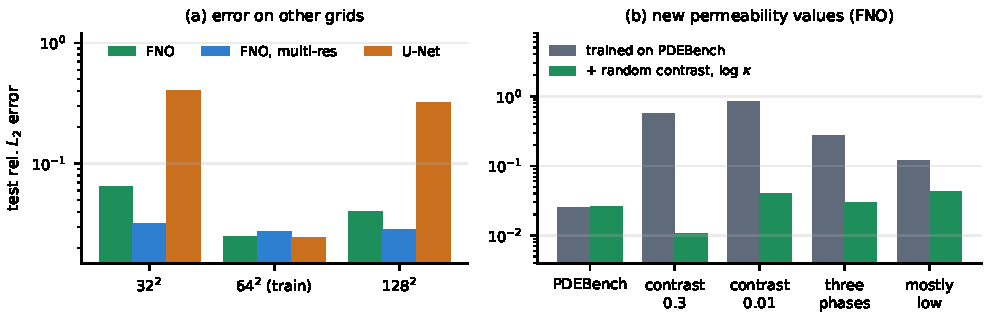
\includegraphics[width=0.98\textwidth]{fig_abstract_v2.pdf}
    \caption{(a) Error on the training grid and on unseen grids, 5\,700 steps, 3 seeds. (b) FNO error on PDEBench and on unseen permeability values, without and with solver-labelled random-contrast data (5\,700 steps, 3 seeds).}
    \label{fig:abs}
\end{figure}
\vspace{-8mm}
\bibliographystyle{unsrt}
\bibliography{references.bib}

\end{document}
